\section{Problem}
\label{sec:problem}

In a typical 3D BPP, a set of items must be packed into fixed-sized bins in the way that minimizes the number of bins used. Unlike typical BPP with fixed-sized bins, we focus on the problem of designing the bin with least surface area that could pack all the items. In real business scenarios, such as cross-board e-commerce, flexible and soft materials are used to fulfill the requirement of  packing all items with no fixed-sized bin. %\kz{According to the problem formulation, the bins are not really soft or flexible, but it's still a rectangular shape box, just with variable L/W/H.} 
After putting the items, the soft and flexible material such as PE bag is similar to rectangular-shaped bin. As the result, the cost of this material is directly proportional to the surface area of the rectangular-shaped bin. In this case, minimizing the surface area for the bin would bring huge economic benefits.

The exact formulation of our problem is shown below. Given a set of cuboid-shaped items and each item $i$ is characterized by length ($l_i$), width ($w_i$) and height ($h_i$). Our target is to find the least-surface-area bin that can pack all items. 
We define $(x_i, y_i, z_i)$ as the left-bottom-back (LBB) coordinate of item 
$i$ and define $(0,0,0)$ as the left-bottom-back coordinate of the bin. 
The details of decision variables are shown in Table \ref{variable table}. 
%\kz{It might be better to have a 3D illustration figure to help explain the constraints in the problem def.}
\begin{table}[th]
	\small
	\centering
	\caption{Decision Variables of New Type of 3D BPP. }
	\label{variable table}
	\begin{tabular}{lll}
		\hline
		Variable           &  Type              & Meaning \\ \hline
		$L$			& Continuous   & the length of the bin                                                                 \\ %\hline   
		$W$			& Continuous   & the width of the bin								 \\ %\hline  
		$H$			& Continuous   & the height of the bin 							\\ %\hline
		$x_{i}$             &   Continuous  & LBB coordinate of item $i$ in $x$ axis        \\ %\hline         
		$y_i$               &   Continuous  &  LBB coordinate of item $i$ in $y$ axis                                                 \\ %\hline
		$z_i$               &   Continuous   & LBB coordinate of item $i$ in $z$ axis             \\ %\hline
		$s_{ij}$	      &    Binary	&  item $i$ is in the left side of item $j$ or not                        \\ %\hline
		$u_{ij}$	      &   Binary         &  item $i$ is under item $j$ or not                                    \\ %\hline
		$b_{ij}$	      &    Binary 	&  item $i$  is in the back of item $j$	or not		\\ %\hline
		${\delta}_{i1}$ &   Binary		&  orientation of item $i$ is front-up or not              \\ %\hline
		${\delta}_{i2}$ &   Binary		&  orientation of item $i$ is front-down or not                       \\ %\hline
		${\delta}_{i3}$ & Binary		&  orientation of item $i$ is side-up or not                      \\ %\hline
		${\delta}_{i4}$ & Binary		&  orientation of item $i$ is side-down or not                   \\ %\hline
		${\delta}_{i5}$ & Binary		&  orientation of item $i$ is bottom-up  or not                      \\ %\hline
		${\delta}_{i6}$ & Binary		&  orientation of item $i$ is bottom-down or not                       \\ \hline
	\end{tabular} 
\end{table}

As shown in the table, we set $s_{ij} = 1$ if item $i$ is in the left side of item $j$, $u_{ij} = 1$ if item $i$ is under item $j$ and $b_{ij} = 1$ if item $i$ is in the back of item $j$.
We also set ${\delta}_{i1} = 1$ if the orientation of item $i$ is front-up, ${\delta}_{i2} = 1$ if the orientation of item $i$ is front-down, ${\delta}_{i3}=1$ if the orientation of item $i$ is side-up, ${\delta}_{i4}=1$ if the orientation of item $i$ is side-down, ${\delta}_{i5} = 1$ if orientations of item $i$ is bottom-up and ${\delta}_{i6} = 1$ if orientation of item $i$ is bottom-down. Consequently, our aim is to find a least surface area bin of which the size is $(L,W,H)$, where $L$, $W$ and $H$ is the length, width and height of the bin, respectively. 

Based on the descriptions of problem and notations, the mathematical formulation for the new type of 3D BPP is followed by \cite{hifi2010linear}:
\begin{eqnarray*}
	\begin{split}
		%\vspace{-100pt}
		%\begin{align*}
		&\min\,\,  L \cdot W + L \cdot H + W \cdot H\\ 
		&\texttt{s}.\texttt{t}.
		\begin{cases}
			s_{ij}+ u_{ij} + b_{ij}  =1          &(1)  \\ %&  i < j = 1,\dots,n    \\
			{\delta}_{i1} + {\delta}_{i2} + {\delta}_{i3} + {\delta}_{i4} + {\delta}_{i5} + {\delta}_{i6} =1  & (2)   \\ 
			x_i - x_j + L  \cdot  s_{ij}  \le  L - \hat{l_i}                           & (3)  \\ %&  i < j = 1,\dots,n \\
			y_i - y_j + W \cdot b_{ij} \le W - \hat{w_i}                        & (4)   \\ %&  i < j = 1,\dots,n \\
			z_i - z_j + H \cdot u_{ij} \le  H - \hat{h_i}                                                                                   & (5)    \\ %&  i < j = 1,\dots,n\\
			0 \le x_i \le L- \hat{l_i}                                     & (6)\\ %&    i = 1,\dots , n      \\
			0 \le y_i \le W - \hat{w_i}                                 & (7)\\ %&      i = 1,\dots , n \\
			0 \le z_i \le H - \hat{h_i}                                   & (8)\\ %&     i = 1,\dots , n  \\
			\hat{l_i} = {\delta}_{i1}   l_i + {\delta}_{i2}  l_i + {\delta}_{i3}  w_i + {\delta}_{i4}  w_i + {\delta}_{i5}  h_i + {\delta}_{i6}  h_i& (9)\\   %&     i = 1,\dots , n \\
			\hat{w_i} = {\delta}_{i1}  w_i +{\delta}_{i2}  h_i +{\delta}_{i3}  l_i +{\delta}_{i4}  h_i +{\delta}_{i5}  l_i +{\delta}_{i6}  w_i& (10)\\ %&     i = 1,\dots , n  \\
			\hat{h_i} =  {\delta}_{i1}  h_i +{\delta}_{i2}  w_i +{\delta}_{i3}  h_i +{\delta}_{i4}  l_i + {\delta}_{i5}  w_i +{\delta}_{i6}  l_i& (11)\\%&     i = 1,\dots , n\\
			s_{ij} , u_{ij},  b_{ij}  \in \{0,1\}                                                                                                                      & (12)\\%&  i < j = 1,\dots,n  \\
			{\delta}_{i1}, {\delta}_{i2}, {\delta}_{i3}, {\delta}_{i4}, {\delta}_{i5}, {\delta}_{i6} \in \{0,1\}                                                     &(13)\\
		\end{cases}
		%\vspace{-20pt}
	\end{split}
\end{eqnarray*}

Constraints $(9) (10) (11)$ denote the length, width, height of item $i$ after orientating it. Constraints $(1) (3) (4) (5)$ are used to guarantee there is no overlap between two packed items while constraints $(6) (7) (8)$ are used to guarantee the item will not be put outside the bin. Figure \ref{fig:problem-illu} explains the non-overlapping constraints in the problem definition.

\begin{figure}[h]
	\centering
	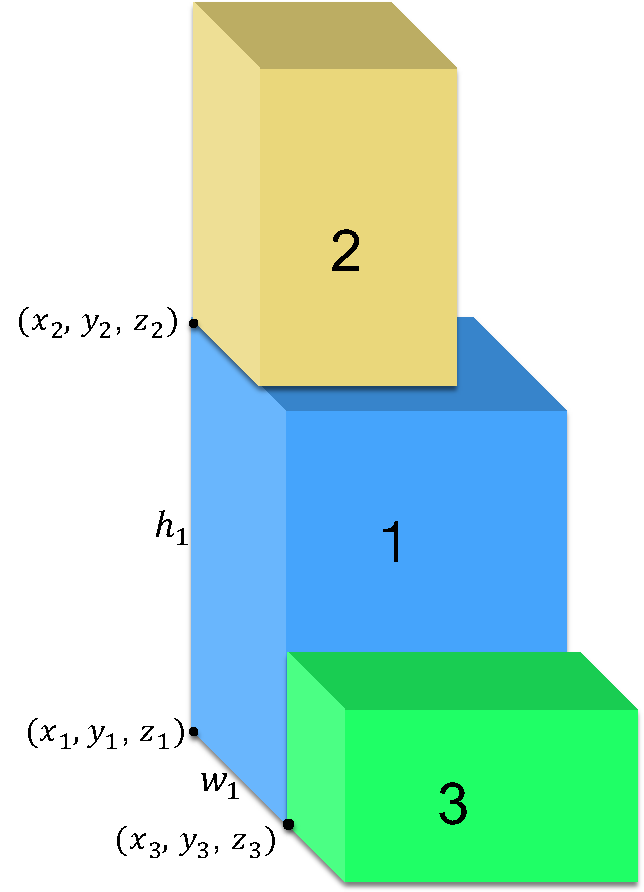
\epsfig{file=problem.pdf, width=0.45\columnwidth}
	\caption{Illustration of non overlapping constraint: item 1 is under item 2 and this means $u_{1,2}=1$ and $z_1 + h_1 <= z_2$, which is condition (5); item 1 is in the back of item 3 and this means $b_{1,3}=1$ and $y_1 + w_1 <= y_3$, which is condition (4). }
	\label{fig:problem-illu}
	\vspace{-10pt}
\end{figure}



We have tried to solve the problem by optimization solvers, such as IBM Cplex Optimizer\footnote{\url{https://www.ibm.com/analytics/data-science/prescriptive-analytics/cplex-optimizer}}, but it is very difficult to solve in reasonable time limit and we will prove this problem is NP-hard in the appendix \ref{np-hard}. 


